\section{Camera Calibration}
In this part we calibrated the camera and then loaded the calibration data that has been stored. Next we calculated the camera matrix for the first view of the calibration.
\begin{equation}
	P_{1} = K
	\begin{bmatrix} R_{1}|t_{1} \end{bmatrix}
\end{equation}
 After these steps we tried to check if P\textsubscript{1} is correct by projecting chesspattern points on the first camera view. As you can see in the \ref{fig:chesspattern} all the points have been projected exactly into the right position.
 
 \begin{figure}[h!]
	\centering
	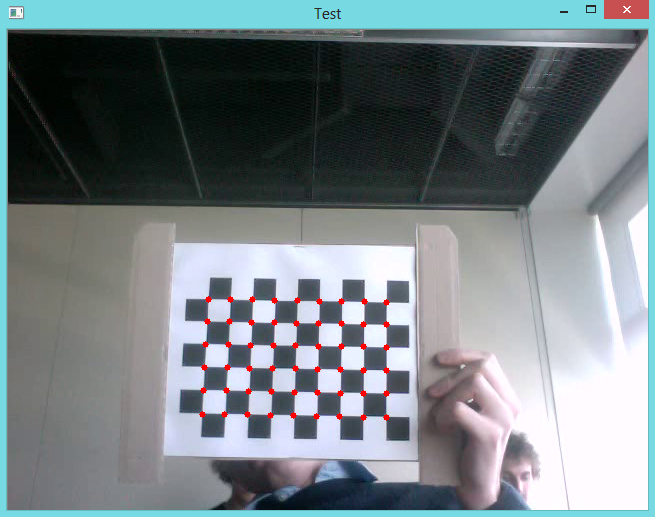
\includegraphics[width=8cm]{Handin3/images/patterndot.jpg}
	\caption{chesspattern}
	\label{fig:chesspattern}
\end{figure}
 
 In the last step of this part we tried to undistort the image by using the (cv2.undistort) function. (see figure \ref{fig:undistort})
 
 \begin{figure}[h!]
	\centering
	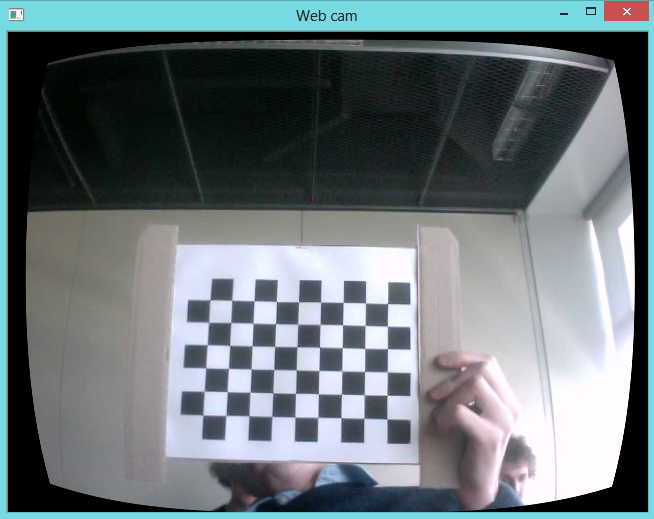
\includegraphics[width=8cm]{Handin3/images/undistort.jpg}
	\caption{undistort}
	\label{fig:undistort}
\end{figure}
 
